% Numerical Integration: from the Trapezoid to Simpson's Rule
% A Beamer presentation with a custom theme (progress bar, section pages, TikZ animations).
\documentclass[aspectratio=169,11pt]{beamer}

\usepackage[T1]{fontenc}
\usepackage[utf8]{inputenc}
\usepackage[sfdefault]{FiraSans}
\usepackage{newtxsf}
\usepackage{amsmath,amssymb}
\usepackage{booktabs,colortbl}
\usepackage{tikz}
\usetikzlibrary{arrows.meta,calc,positioning}
\usepackage{pgfplots}
\pgfplotsset{compat=1.18}
\usepackage{algorithmicx,algpseudocode}
\usepackage{listings}
\usepackage[backend=biber,style=numeric,sorting=none]{biblatex}
\addbibresource{references.bib}

% ---------------------------------------------------------------- colours
\definecolor{navy}{HTML}{0B2545}
\definecolor{tealc}{HTML}{13A89E}
\definecolor{amberc}{HTML}{F4B942}
\definecolor{coral}{HTML}{E4572E}

\setbeamercolor{normal text}{fg=navy!90!black,bg=white}
\setbeamercolor{structure}{fg=tealc!80!black}
\setbeamercolor{frametitle}{fg=navy}
\setbeamercolor{block title}{bg=navy,fg=white}
\setbeamercolor{block body}{bg=navy!6,fg=black}
\setbeamercolor{block title example}{bg=tealc!80!black,fg=white}
\setbeamercolor{block body example}{bg=tealc!9,fg=black}
\setbeamercolor{block title alerted}{bg=coral,fg=white}
\setbeamercolor{block body alerted}{bg=coral!8,fg=black}
\setbeamercolor{alerted text}{fg=coral}
\setbeamercolor{footline}{fg=navy!55}

% ---------------------------------------------------------------- templates
\setbeamertemplate{navigation symbols}{}
\setbeamertemplate{blocks}[rounded][shadow=false]
\setbeamertemplate{itemize items}[circle]
\setbeamertemplate{bibliography item}[text]
\setbeamersize{text margin left=1.6em,text margin right=1.6em}
\setbeamerfont{frametitle}{size=\Large,series=\bfseries}
\setbeamerfont{footline}{size=\scriptsize}
\setbeamerfont{block title}{series=\bfseries,size=\normalsize}

\setbeamertemplate{frametitle}{%
  \vspace{0.5em}%
  \begin{beamercolorbox}[wd=\paperwidth,leftskip=1.6em]{frametitle}%
    \usebeamerfont{frametitle}\insertframetitle\par
    \vspace{-0.3em}\tikz{\fill[tealc] (0,0) rectangle (1.8,0.07);}%
  \end{beamercolorbox}}

\newdimen\barw
\setbeamertemplate{headline}{%
  \global\barw=\dimexpr\paperwidth*\insertframenumber/\inserttotalframenumber\relax
  
\begin{tikzpicture}[overlay]
    \fill[navy!10] (0,-3pt) rectangle (\paperwidth,0);
    \fill[tealc]   (0,-3pt) rectangle (\barw,0);
  \end{tikzpicture}}

\setbeamertemplate{footline}{%
  \leavevmode\hbox{\begin{beamercolorbox}[wd=\paperwidth,ht=2.6ex,dp=1.4ex,leftskip=1.6em,rightskip=1.6em]{footline}%
    \usebeamerfont{footline}\insertshortauthor\hfill\insertshorttitle\hfill\insertframenumber/\inserttotalframenumber
  \end{beamercolorbox}}}

% title page
\setbeamertemplate{title page}{%
  
\begin{tikzpicture}[remember picture,overlay]
    \fill[navy] (current page.south west) rectangle (current page.north east);
    \draw[white,opacity=0.05,step=1cm] (current page.south west) grid (current page.north east);
    \begin{scope}[shift={(current page.south east)},xshift=-6.4cm,yshift=1.4cm,scale=0.66]
      \draw[white,opacity=0.35,->] (0,0) -- (8.4,0);
      \draw[white,opacity=0.35,->] (0,0) -- (0,5.4);
      \foreach \i in {0,...,5}{%
        \pgfmathsetmacro{\xa}{\i*1.3}\pgfmathsetmacro{\xb}{(\i+1)*1.3}%
        \pgfmathsetmacro{\ya}{4.8*exp(-(\i/5)^2)}\pgfmathsetmacro{\yb}{4.8*exp(-((\i+1)/5)^2)}%
        \fill[tealc,opacity=0.22] (\xa,0) -- (\xa,\ya) -- (\xb,\yb) -- (\xb,0) -- cycle;
        \draw[tealc,opacity=0.7] (\xa,0) -- (\xa,\ya) -- (\xb,\yb) -- (\xb,0);}
      \draw[amberc,very thick,domain=0:7.8,samples=60] plot (\x,{4.8*exp(-(\x/6.5)^2)});
    \end{scope}
    \node[anchor=west,text width=0.56\paperwidth,white,align=left] at ([xshift=1.6cm,yshift=0.9cm]current page.west)
      {\hyphenpenalty=10000\exhyphenpenalty=10000{\fontsize{32}{36}\selectfont\bfseries\inserttitle\par}\vspace{0.4cm}%
       {\Large\color{tealc!60!white}\insertsubtitle\par}\vspace{1.1cm}%
       {\large\bfseries\insertauthor\par}\vspace{2pt}%
       {\normalsize\color{white!75!navy}\insertinstitute\par}\vspace{2pt}%
       {\normalsize\color{white!75!navy}\insertdate\par}};
  \end{tikzpicture}}

% section pages
\setbeamertemplate{section page}{%
  \begin{tikzpicture}[remember picture,overlay]
    \fill[navy] (current page.south west) rectangle (current page.north east);
    \node[anchor=west,tealc,font=\fontsize{70}{70}\selectfont\bfseries] at ([xshift=1.8cm]current page.west) {\thesection};
    \node[anchor=west,white,font=\fontsize{30}{34}\selectfont\bfseries,text width=0.62\paperwidth] at ([xshift=4.6cm]current page.west) {\hyphenpenalty=10000\exhyphenpenalty=10000 \insertsectionhead};
    \fill[amberc] ([xshift=4.6cm,yshift=-1.75cm]current page.west) rectangle ++(2.2,0.08);
  \end{tikzpicture}}
\AtBeginSection{\begin{frame}[plain,noframenumbering]\sectionpage\end{frame}}

% ---------------------------------------------------------------- helpers
\lstset{language=Python,basicstyle=\ttfamily\footnotesize,keywordstyle=\color{tealc!70!black}\bfseries,
  commentstyle=\color{gray}\itshape,stringstyle=\color{coral},showstringspaces=false,
  frame=single,rulecolor=\color{navy!20},backgroundcolor=\color{navy!3},numbers=left,
  numberstyle=\tiny\color{gray},xleftmargin=1.6em,columns=fullflexible}

\algrenewcommand\algorithmicrequire{\textbf{Input:}}
\algrenewcommand\algorithmicensure{\textbf{Output:}}

% draw n trapezoids of f(x)=exp(-x^2) on [0,1] inside a pgfplots axis
\newcommand{\trapezoids}[1]{%
  \pgfmathtruncatemacro{\nm}{#1-1}%
  \foreach \i in {0,...,\nm}{%
    \pgfmathsetmacro{\xa}{\i/#1}\pgfmathsetmacro{\xb}{(\i+1)/#1}%
    \pgfmathsetmacro{\ya}{exp(-\xa*\xa)}\pgfmathsetmacro{\yb}{exp(-\xb*\xb)}%
    \addplot[draw=tealc!70!black,fill=tealc!22] coordinates {(\xa,0) (\xa,\ya) (\xb,\yb) (\xb,0)} \closedcycle;%
  }}

\title[Numerical Integration]{Numerical Integration}
\subtitle{From the Trapezoid to Simpson's Rule}
\author[N.\,S. Yamontche]{N'sol\'e Samson Yamontche}
\institute{UNSTIM, Benin}
\date{October 2026}

\begin{document}
\hyphenpenalty=10000 \exhyphenpenalty=10000 \tolerance=2000 \emergencystretch=2em

\begin{frame}[plain,noframenumbering]
  \titlepage
\end{frame}

% ================================================================ outline
\begin{frame}{Outline}
  \tableofcontents
\end{frame}

% ================================================================ 1
\section{Why integrate numerically?}

\begin{frame}{Integrals we cannot solve by hand}
  \begin{columns}[T]
    \begin{column}{0.52\textwidth}
      \begin{itemize}
        \setlength\itemsep{0.8em}
        \item<1-> Many integrands have \alert{no elementary antiderivative}:
          \[ \int e^{-x^{2}}\,\mathrm{d}x, \qquad \int \frac{\sin x}{x}\,\mathrm{d}x \]
        \item<2-> Data often come as a \alert{table of values}, not as a formula.
        \item<3-> Physics and engineering need numbers: work, probability, signal energy.
      \end{itemize}
    \end{column}
    \begin{column}{0.46\textwidth}
      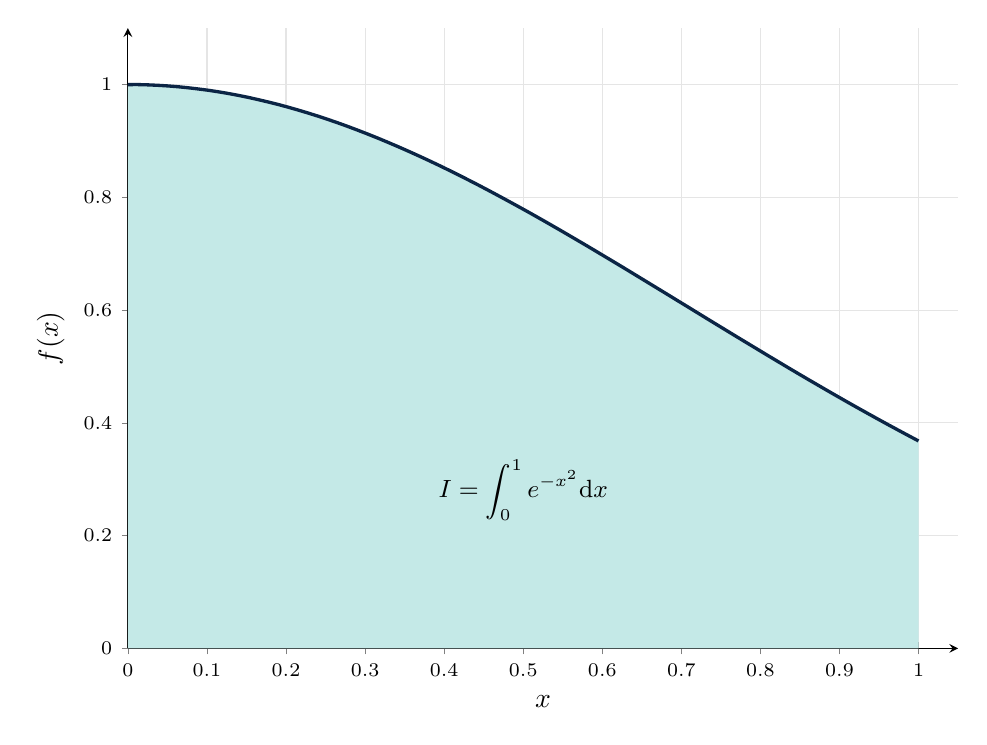
\begin{tikzpicture}
        \begin{axis}[width=\linewidth,height=0.78\linewidth,xlabel={$x$},ylabel={$f(x)$},axis lines=left,
            xmin=0,xmax=1.05,ymin=0,ymax=1.1,tick label style={font=\scriptsize},grid=both,grid style={gray!20}]
          \addplot[draw=none,fill=tealc!25,domain=0:1,samples=60] {exp(-x^2)} \closedcycle;
          \addplot[navy,very thick,domain=0:1,samples=80] {exp(-x^2)};
          \node[font=\small] at (axis cs:0.5,0.28) {$I=\displaystyle\int_0^1 e^{-x^2}\mathrm{d}x$};
        \end{axis}
      \end{tikzpicture}
    \end{column}
  \end{columns}
  \vspace{0.3em}
  \onslide<4->{\begin{exampleblock}{Our running example}
    $I=\dfrac{\sqrt{\pi}}{2}\operatorname{erf}(1)\approx 0.7468241328$ \quad (exact value, used to measure the errors)
  \end{exampleblock}}
\end{frame}

% ================================================================ 2
\section{The trapezoidal rule}

\begin{frame}{Replace the curve by straight segments}
  \begin{columns}[T]
    \begin{column}{0.44\textwidth}
      Split $[a,b]$ into $n$ equal pieces of width $h=\dfrac{b-a}{n}$ and approximate $f$ by a line on each piece:
      \[
        T_n = h\left[\tfrac12 f(a) + \sum_{i=1}^{n-1} f(x_i) + \tfrac12 f(b)\right]
      \]
      \vspace{-0.3em}
      \begin{block}{Refine the mesh}
        \only<1>{$n=2$ \quad error $\approx 1.5\cdot10^{-2}$}%
        \only<2>{$n=4$ \quad error $\approx 3.8\cdot10^{-3}$}%
        \only<3>{$n=8$ \quad error $\approx 9.6\cdot10^{-4}$}%
      \end{block}
    \end{column}
    \begin{column}{0.54\textwidth}
      \begin{tikzpicture}
        \begin{axis}[width=\linewidth,height=0.72\linewidth,xlabel={$x$},axis lines=left,xmin=0,xmax=1.05,ymin=0,ymax=1.1,
            tick label style={font=\scriptsize},grid=both,grid style={gray!20}]
          \only<1>{\trapezoids{2}}
          \only<2>{\trapezoids{4}}
          \only<3>{\trapezoids{8}}
          \addplot[navy,very thick,domain=0:1,samples=80] {exp(-x^2)};
        \end{axis}
      \end{tikzpicture}
    \end{column}
  \end{columns}
\end{frame}

\begin{frame}{How accurate is it?}
  \begin{theorem}[Trapezoidal error]
    If $f\in C^{2}[a,b]$, then
    \[
      \lvert I-T_n\rvert \le \frac{(b-a)\,h^{2}}{12}\,\max_{[a,b]}\lvert f''\rvert .
    \]
  \end{theorem}
  \pause
  \begin{itemize}
    \setlength\itemsep{0.6em}
    \item The error decreases like $h^{2}$: \alert{doubling $n$ divides the error by about $4$}.
    \item The rule is exact for every polynomial of degree $\le 1$.
  \end{itemize}
\end{frame}

% ================================================================ 3
\section{Simpson's rule}

\begin{frame}{Replace the curve by parabolas}
  \begin{columns}[T]
    \begin{column}{0.46\textwidth}
      On each pair of pieces, fit a parabola through three points. For $n=2$:
      \[ S_2=\frac{h}{3}\bigl[f(x_0)+4f(x_1)+f(x_2)\bigr] \]
      \vspace{-0.2em}
      \onslide<2->{%
      \begin{exampleblock}{Check}
        $h=\tfrac12$ gives $S_2=\tfrac16(1+4e^{-1/4}+e^{-1})\approx 0.74718$
      \end{exampleblock}}
    \end{column}
    \begin{column}{0.52\textwidth}
      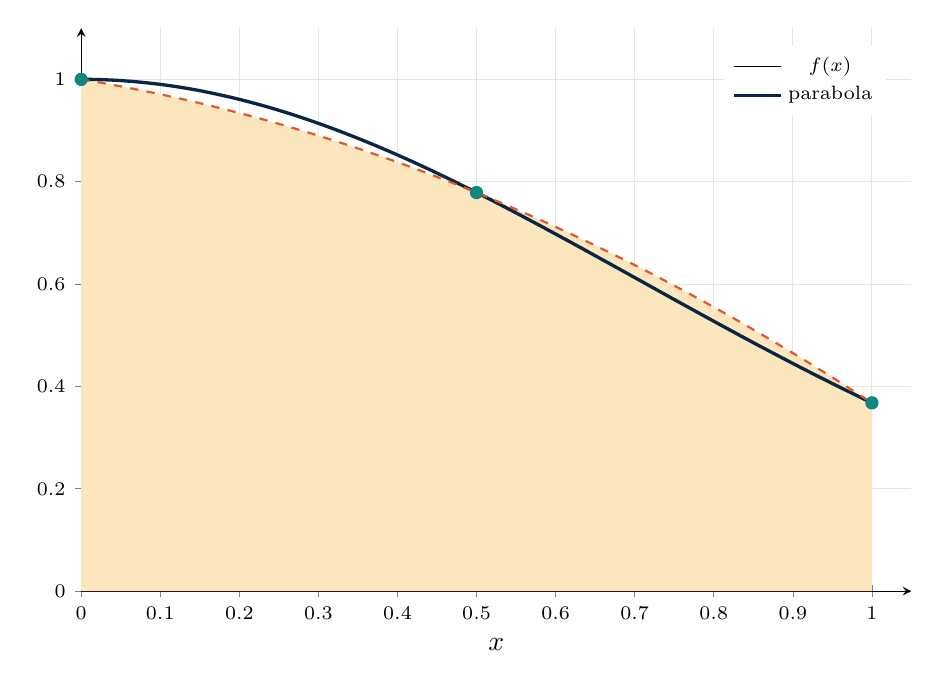
\begin{tikzpicture}
        \begin{axis}[width=\linewidth,height=0.72\linewidth,xlabel={$x$},axis lines=left,xmin=0,xmax=1.05,ymin=0,ymax=1.1,
            tick label style={font=\scriptsize},grid=both,grid style={gray!20},legend style={font=\scriptsize,draw=none,at={(0.97,0.97)},anchor=north east}]
          \onslide<2->{\addplot[draw=none,fill=amberc!35,domain=0:1,samples=40] {1-0.252675*x-0.379446*x^2} \closedcycle;}
          \addplot[navy,very thick,domain=0:1,samples=80] {exp(-x^2)};
          \addlegendentry{$f(x)$}
          \addplot[coral,thick,dashed,domain=0:1,samples=40] {1-0.252675*x-0.379446*x^2};
          \addlegendentry{parabola}
          \addplot[only marks,mark=*,mark size=2.2pt,tealc!80!black] coordinates {(0,1) (0.5,0.778801) (1,0.367879)};
        \end{axis}
      \end{tikzpicture}
    \end{column}
  \end{columns}
\end{frame}

\begin{frame}{The composite rule and its error}
  For an even number $n$ of pieces:
  \[
    S_n=\frac{h}{3}\Bigl[f(x_0)+4\!\!\sum_{i\ \mathrm{odd}}\!\! f(x_i)+2\!\!\sum_{\substack{i\ \mathrm{even}\\ 2\le i\le n-2}}\!\! f(x_i)+f(x_n)\Bigr]
  \]
  \begin{theorem}[Simpson error]
    If $f\in C^{4}[a,b]$, then $\displaystyle\lvert I-S_n\rvert \le \frac{(b-a)\,h^{4}}{180}\,\max_{[a,b]}\lvert f^{(4)}\rvert$.
  \end{theorem}
  \pause
  \begin{alertblock}{Consequence}
    The error decreases like $h^{4}$: \textbf{doubling $n$ divides the error by about $16$.}
    Simpson's rule is exact for polynomials up to degree $3$.
  \end{alertblock}
\end{frame}

% ================================================================ 4
\section{Implementation}

\begin{frame}{The algorithm}
  \begin{columns}[T]
    \begin{column}{0.55\textwidth}
      \begin{algorithmic}[1]
        \Require function $f$, interval $[a,b]$, even integer $n$
        \Ensure approximation $S_n$ of $\int_a^b f$
        \State $h \gets (b-a)/n$
        \State $s \gets f(a)+f(b)$
        \For{$i=1$ \textbf{to} $n-1$}
          \If{$i$ is odd}
            \State $s \gets s+4f(a+ih)$
          \Else
            \State $s \gets s+2f(a+ih)$
          \EndIf
        \EndFor
        \State \Return $h\,s/3$
      \end{algorithmic}
    \end{column}
    \begin{column}{0.41\textwidth}
      \begin{block}{Cost}
        $n+1$ evaluations of $f$ and $O(n)$ operations.
      \end{block}
      \begin{exampleblock}{Tip}
        Choose $n$ even, and double it until two successive results agree.
      \end{exampleblock}
    \end{column}
  \end{columns}
\end{frame}

\begin{frame}[fragile]{The same algorithm in Python}
\begin{lstlisting}
import math

def simpson(f, a, b, n):
    if n % 2:
        raise ValueError("n must be even")
    h = (b - a) / n
    s = f(a) + f(b)
    s += 4 * sum(f(a + i*h) for i in range(1, n, 2))
    s += 2 * sum(f(a + i*h) for i in range(2, n-1, 2))
    return s * h / 3

print(simpson(lambda x: math.exp(-x*x), 0, 1, 16))
# 0.7468242574357303
\end{lstlisting}
\end{frame}

% ================================================================ 5
\section{Experiments}

\begin{frame}{Numerical results}
  \centering
  \renewcommand{\arraystretch}{1.25}
  \begin{tabular}{r c c c c}
    \toprule
    \rowcolor{navy!8} $n$ & $T_n$ & $S_n$ & $\lvert I-T_n\rvert$ & $\lvert I-S_n\rvert$ \\
    \midrule
     2 & 0.731370 & 0.747180 & $1.545\cdot10^{-2}$ & $3.563\cdot10^{-4}$ \\
     4 & 0.742984 & 0.746855 & $3.840\cdot10^{-3}$ & $3.125\cdot10^{-5}$ \\
     8 & 0.745866 & 0.746826 & $9.585\cdot10^{-4}$ & $1.988\cdot10^{-6}$ \\
    \rowcolor{tealc!12}
    16 & 0.746585 & 0.746824 & $2.395\cdot10^{-4}$ & $1.246\cdot10^{-7}$ \\
    \bottomrule
  \end{tabular}

  \vspace{1em}
  \begin{minipage}{0.8\textwidth}\centering
    Exact value: $I\approx 0.7468241328$. With only $n=16$, Simpson's rule is accurate to seven digits.
  \end{minipage}
\end{frame}

\begin{frame}{Convergence study}
  \begin{columns}[T]
    \begin{column}{0.62\textwidth}
      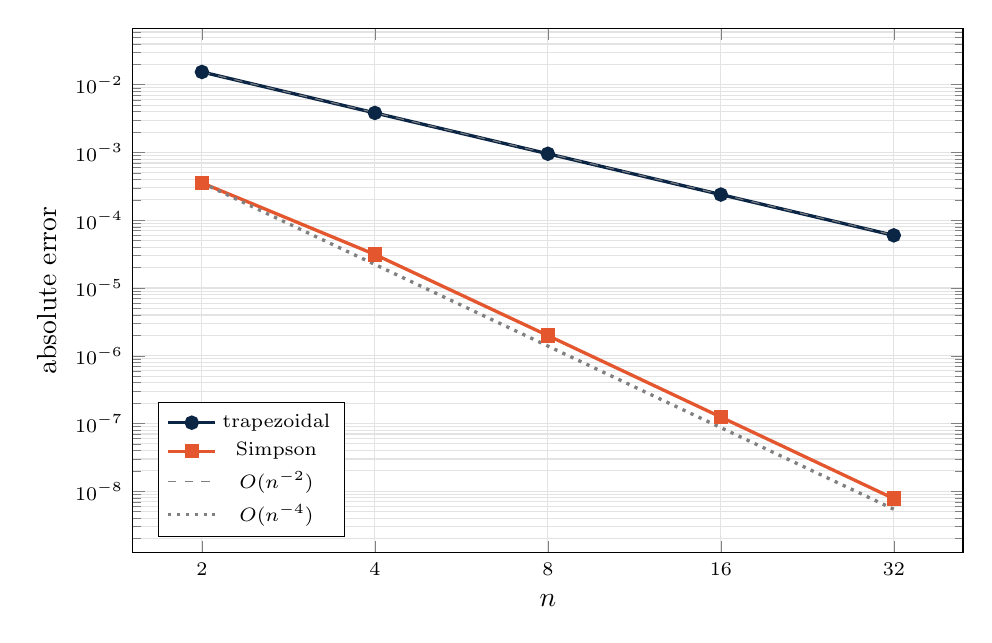
\begin{tikzpicture}
        \begin{axis}[width=\linewidth,height=0.68\linewidth,xmode=log,ymode=log,log basis x=2,
            xtick={2,4,8,16,32},xticklabels={2,4,8,16,32},xlabel={$n$},ylabel={absolute error},
            grid=both,grid style={gray!22},legend pos=south west,legend style={font=\scriptsize},tick label style={font=\scriptsize}]
          \addplot[navy,mark=*,very thick] coordinates {(2,1.545e-2) (4,3.840e-3) (8,9.585e-4) (16,2.395e-4) (32,5.988e-5)};
          \addlegendentry{trapezoidal}
          \onslide<2->{\addplot[coral,mark=square*,very thick] coordinates {(2,3.563e-4) (4,3.125e-5) (8,1.988e-6) (16,1.246e-7) (32,7.795e-9)};
          \addlegendentry{Simpson}}
          \onslide<3->{\addplot[gray,dashed,domain=2:32] {1.545e-2*(2/x)^2};
          \addlegendentry{$O(n^{-2})$}
          \addplot[gray,dotted,very thick,domain=2:32] {3.563e-4*(2/x)^4};
          \addlegendentry{$O(n^{-4})$}}
        \end{axis}
      \end{tikzpicture}
    \end{column}
    \begin{column}{0.34\textwidth}
      \vspace{1em}
      \begin{itemize}
        \setlength\itemsep{0.9em}
        \item<1-> Trapezoidal: slope $-2$.
        \item<2-> Simpson: slope $-4$.
        \item<3-> The measured slopes \alert{match the theory}.
      \end{itemize}
    \end{column}
  \end{columns}
\end{frame}

\begin{frame}{Which rule should I use?}
  \begin{columns}[T]
    \begin{column}{0.48\textwidth}
      \begin{block}{Trapezoidal rule}
        \begin{itemize}
          \item very simple
          \item works with any $n$
          \item order $h^{2}$
          \item good for \alert{periodic} integrands
        \end{itemize}
      \end{block}
    \end{column}
    \begin{column}{0.48\textwidth}
      \begin{exampleblock}{Simpson's rule}
        \begin{itemize}
          \item same cost per evaluation
          \item needs an even $n$
          \item order $h^{4}$
          \item best for \alert{smooth} integrands
        \end{itemize}
      \end{exampleblock}
    \end{column}
  \end{columns}
\end{frame}

% ================================================================ 6
\section{Conclusion}

\begin{frame}{Take-home messages}
  \large
  \begin{enumerate}
    \setlength\itemsep{0.9em}
    \item<1-> Numerical integration replaces $f$ by simple pieces: \alert{lines} or \alert{parabolas}.
    \item<2-> Error orders: $O(h^{2})$ for the trapezoid, $O(h^{4})$ for Simpson.
    \item<3-> On $\int_0^1 e^{-x^{2}}\mathrm{d}x$, $n=16$ gives \alert{$2\cdot10^{-4}$} versus \alert{$1\cdot10^{-7}$}.
    \item<4-> Always check convergence by doubling $n$.
  \end{enumerate}
\end{frame}

\begin{frame}[allowframebreaks]{References}
  \nocite{burden2016,atkinson1989,press2007}
  \printbibliography[heading=none]
\end{frame}

\begin{frame}[plain,noframenumbering]
  \begin{tikzpicture}[remember picture,overlay]
    \fill[navy] (current page.south west) rectangle (current page.north east);
    \node[white,font=\fontsize{40}{44}\selectfont\bfseries] at ([yshift=1.0cm]current page.center) {Thank you};
    \node[tealc!60!white,font=\Large] at ([yshift=-0.2cm]current page.center) {Questions?};
    \node[white!75!navy,font=\normalsize] at ([yshift=-1.6cm]current page.center) {N'sol\'e Samson Yamontche \quad\textbullet\quad samsonyamontchensolegit.github.io};
  \end{tikzpicture}
\end{frame}

\end{document}
